\chapter{Evaluation and Experiments}

This chapter describes the evaluation methodology and outlines the metrics and figures that will be used to quantify the performance of our learned policies on both single-quadrotor and multi-quadrotor cable-suspended payload transport tasks.

\section{Experimental Setup}
We first evaluate the performance of our learned policies in our simulation environment. We use only the actor network for evaluation, as the critic is not needed for inference. The policies are trained using the \gls{ippo} algorithm.
All experiments were conducted in simulation using a policy frequency of 250 Hz with one physics step per control action. We set both observation and actuator noise to zero, randomized thrust within $0.2$, used a 0.4 m cable length, and fixed the payload mass at 0.01 kg. 

Two primary tasks were evaluated: a real-time figure-eight trajectory tracking task and a recovery-from-harsh-conditions task. In the figure-eight tracking task, each episode ran for 5,000 steps, the payload followed a precomputed figure-eight path, and the quadrotor always initialized at the center, with performance aggregated over 100 rollouts. In the recovery task, episodes lasted 2,500 steps, the payload target remained fixed at $(0 0 1.5)$ m, and the agent began from random harsh initial states. metrics were gathered over 1,000 rollouts. For multi-quadrotor experiments, policies for teams of two, three, and five quadrotors were evaluated, with each quadrotor initialized at the target position and the payload suspended at the center of mass of the quadrotors as explained in seciton \todo{ref}. The payload was always initialized at $(0 0 1.5)$ m, and the quadrotors were positioned in a circle around it.

\section{Single-Quadrotor Payload Control}
We first evaluate the learned policy on the single-vehicle case, testing both disturbance recovery and trajectory tracking on a figure-eight path. See Figure \ref{fig:single_quad_payload_subfigs}.
The experiments demonstrate the quadrotor's ability to recover from harsh conditions and disturbances in under 2 seconds. 

\begin{figure}[ht]
    \centering
    \begin{subfigure}[b]{0.49\textwidth}
        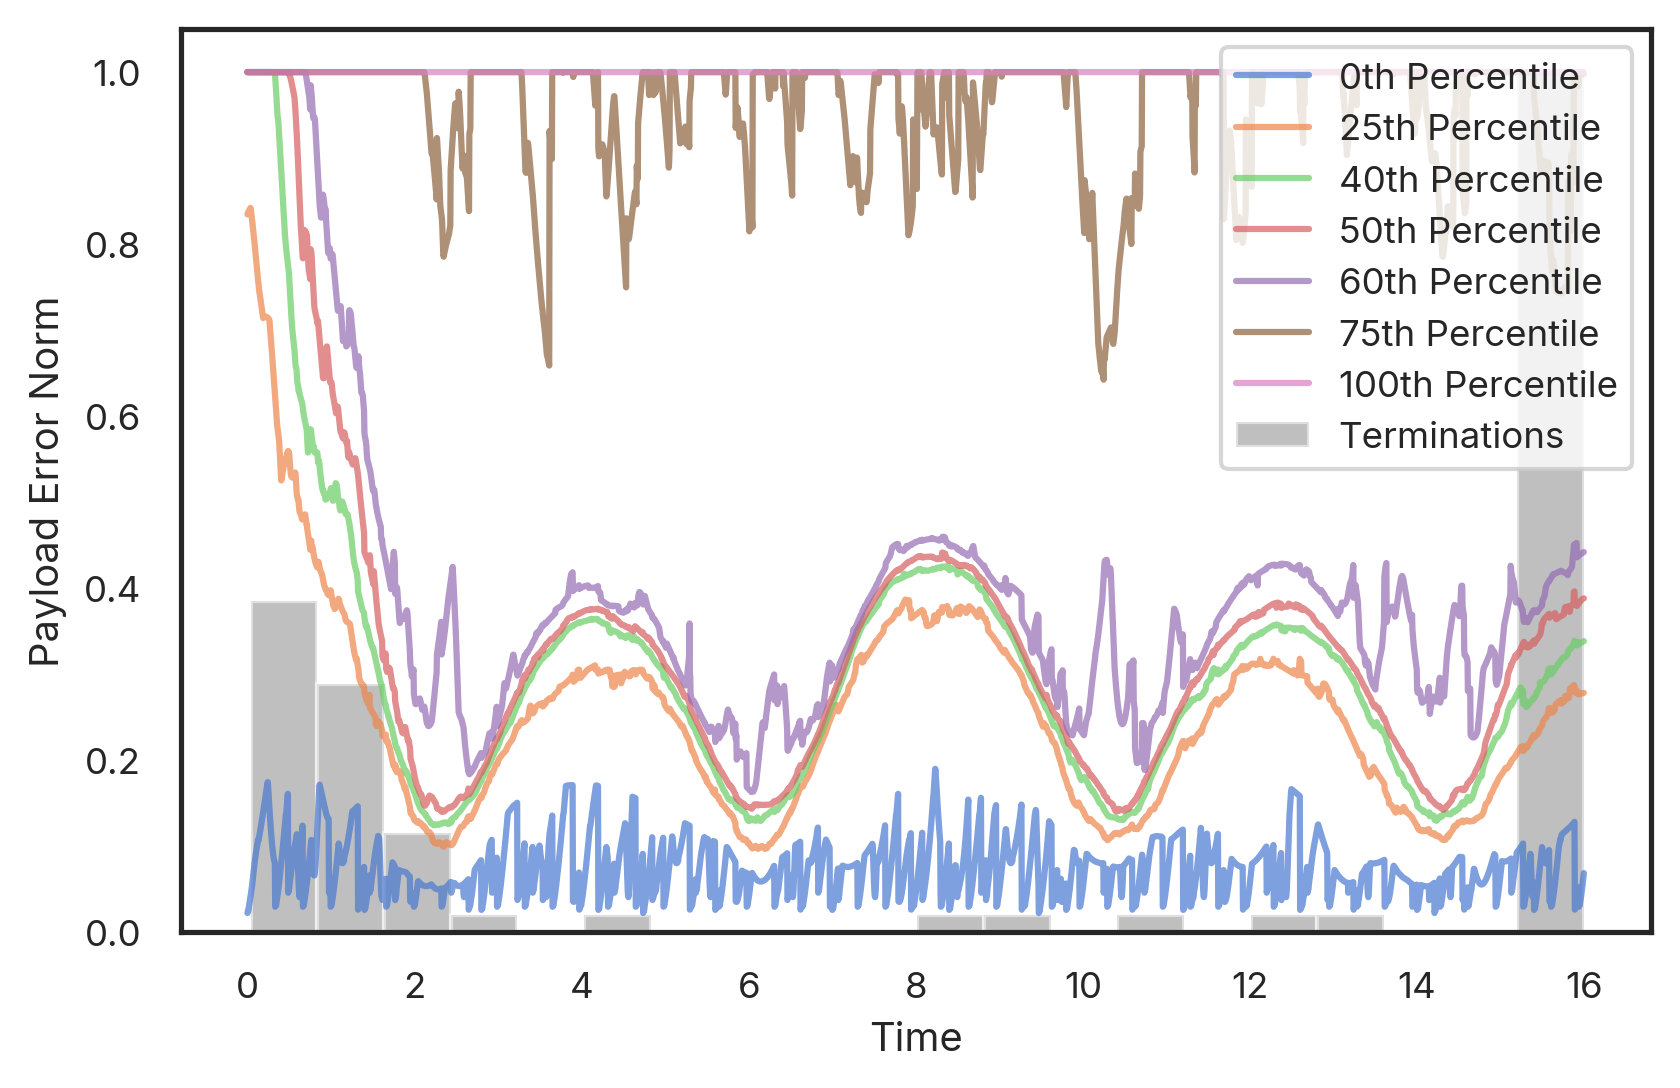
\includegraphics[width=\textwidth]{experiments/payload_error_over_time.png}
        \caption{Positional error over time across 1,000 rollouts.}
        \label{fig:payload_error_over_time}
    \end{subfigure}
    \hfill
    \begin{subfigure}[b]{0.49\textwidth}
        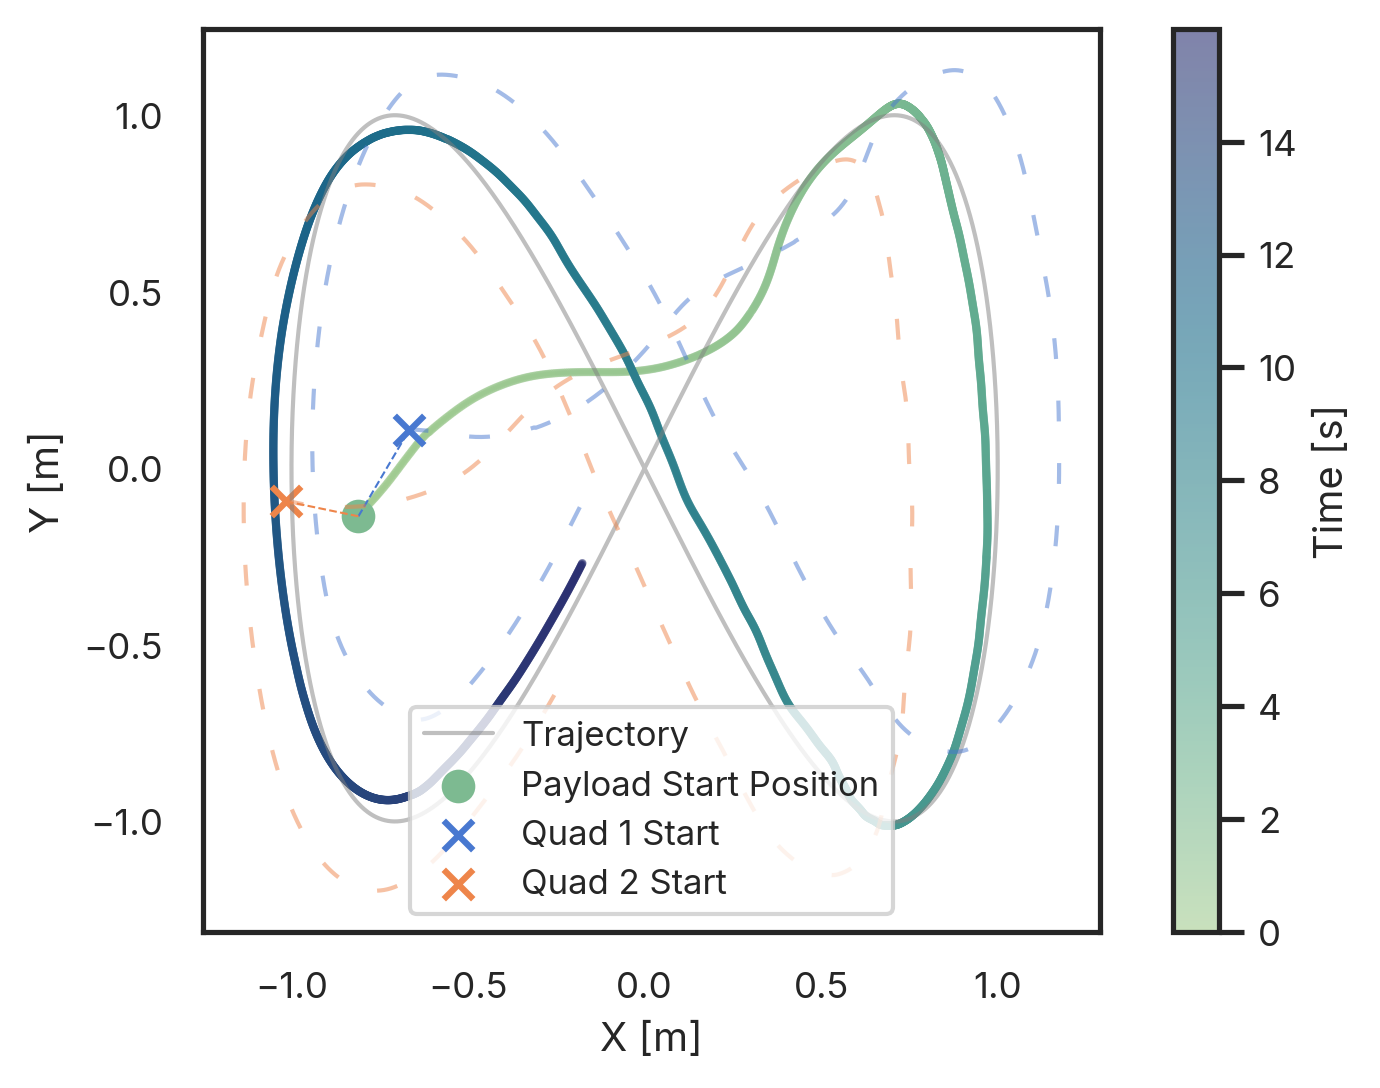
\includegraphics[width=\textwidth]{experiments/payload_position_xy.png}
        \caption{XY trajectory on a figure-eight path.}
        \label{fig:payload_position_xy}
    \end{subfigure}
    \caption{Performance of a single quadrotor carrying a suspended payload: disturbance recovery and trajectory tracking.}
    \label{fig:single_quad_payload_subfigs}
\end{figure}

\section{Multi-Quadrotor Payload Transport}
We extend the evaluation to cooperative transport tasks involving teams of two, three, and five quadrotors to demonstrate scalability. See Figure \ref{fig:multi_quad_payload}.

\begin{figure}[ht]
    \centering
    % Two quadrotors
    \begin{subfigure}[b]{0.49\textwidth}
        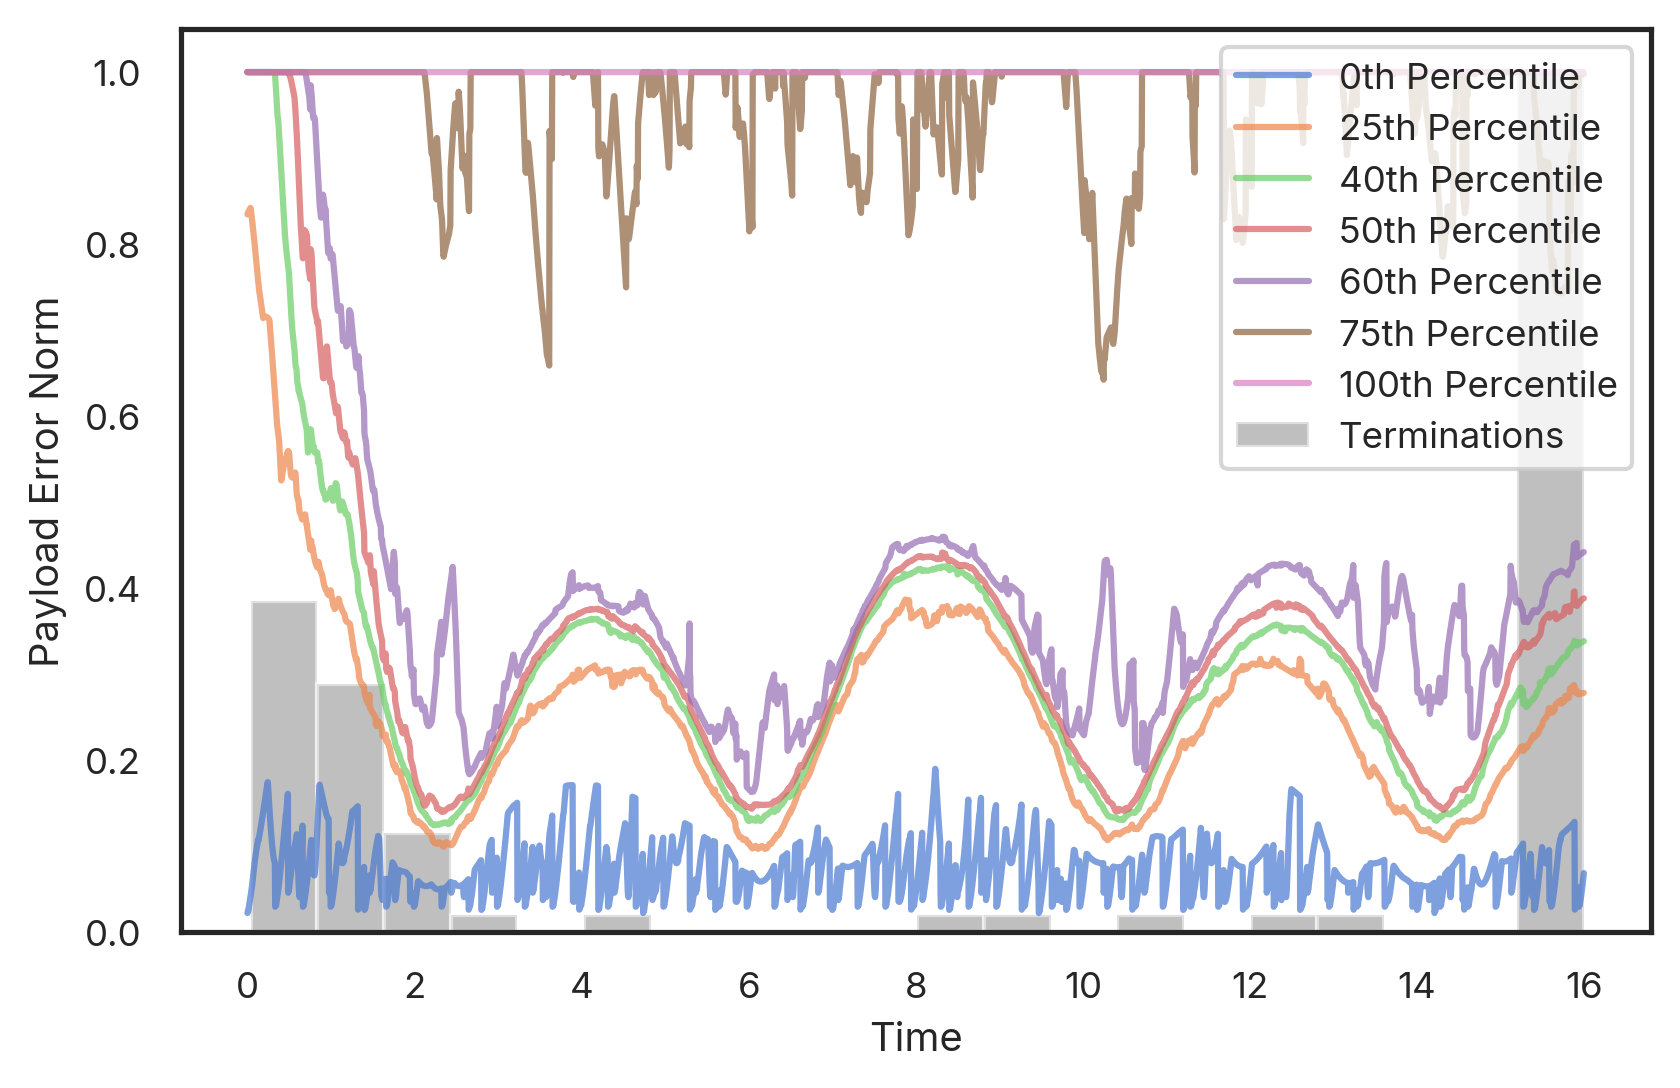
\includegraphics[width=\textwidth]{experiments/payload_error_over_time.png}
        \caption{2 agents: positional error over time (1,000 rollouts).}
        \label{fig:payload_error_2quads}
    \end{subfigure}
    \hfill
    \begin{subfigure}[b]{0.49\textwidth}
        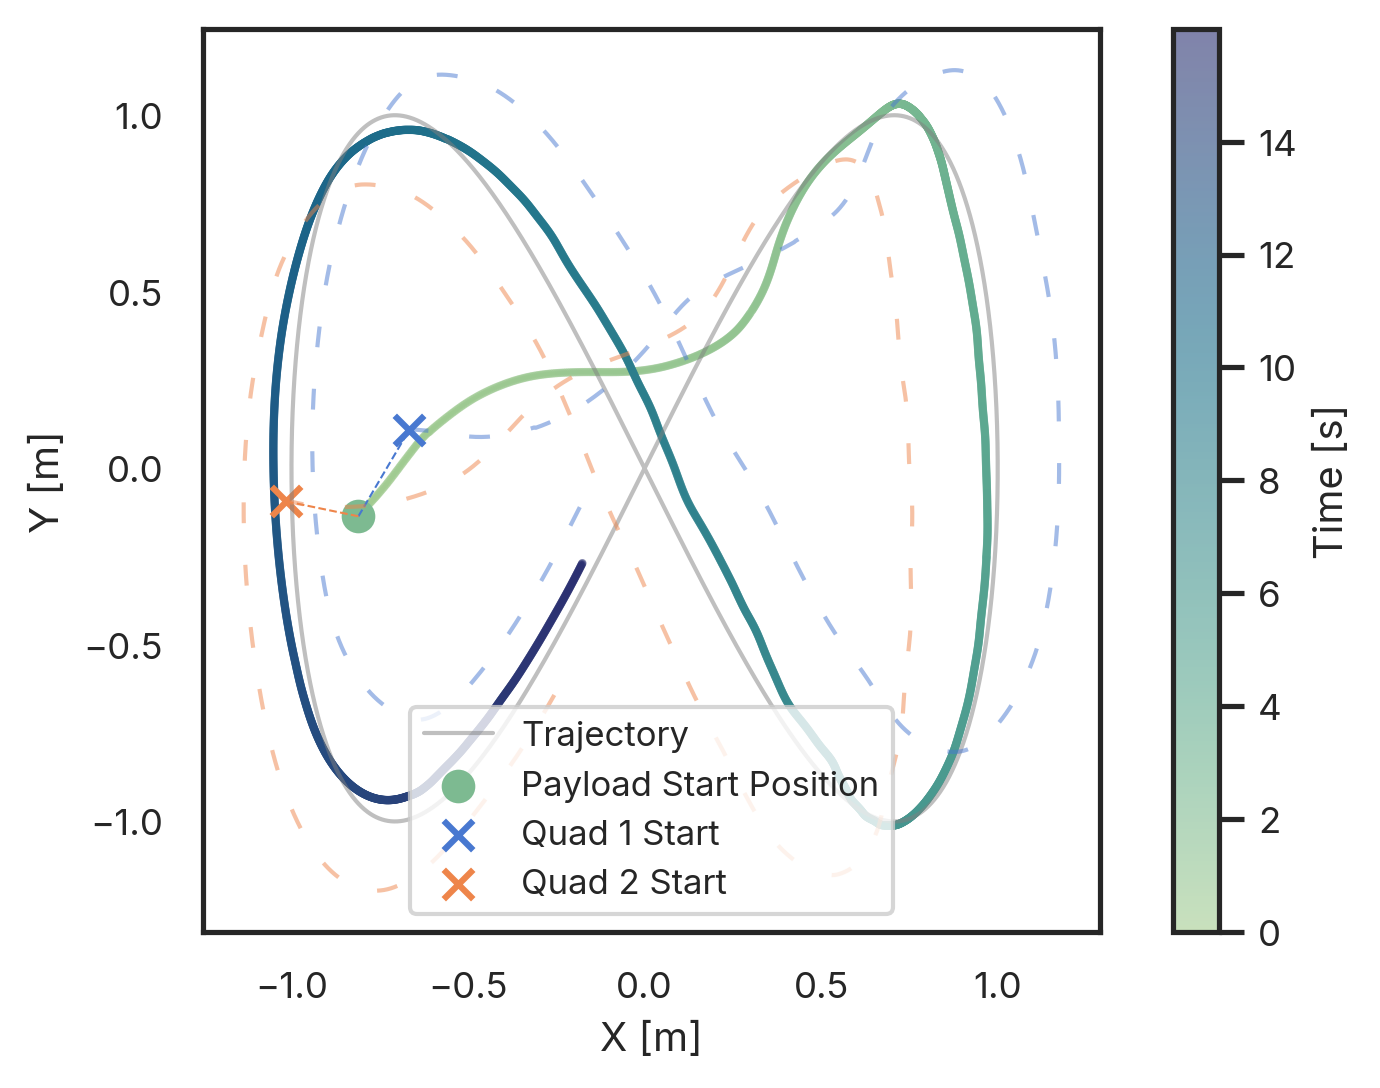
\includegraphics[width=\textwidth]{experiments/payload_position_xy.png}
        \caption{2 agents: figure-eight tracking.}
        \label{fig:payload_position_2quads}
    \end{subfigure}

    \vspace{1em}

    % Three quadrotors
    \begin{subfigure}[b]{0.49\textwidth}
        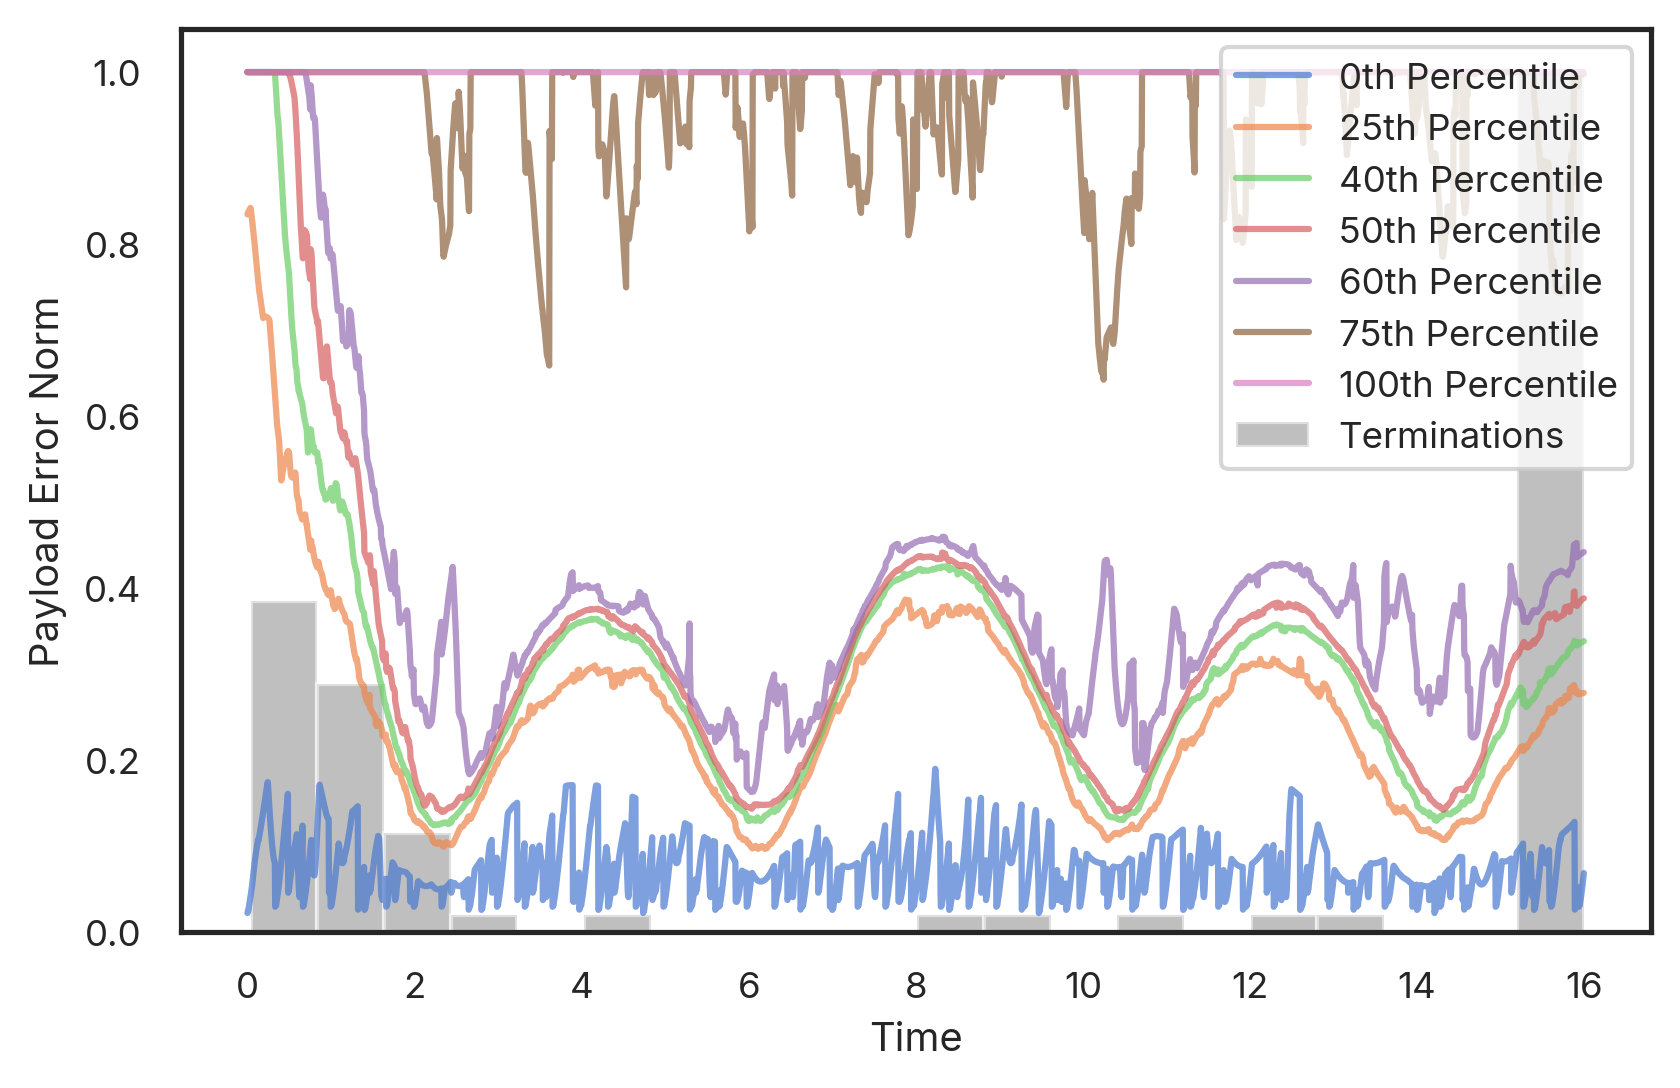
\includegraphics[width=\textwidth]{experiments/payload_error_over_time.png}
        \caption{3 agents: positional error over time (1,000 rollouts).}
        \label{fig:payload_error_3quads}
    \end{subfigure}
    \hfill
    \begin{subfigure}[b]{0.49\textwidth}
        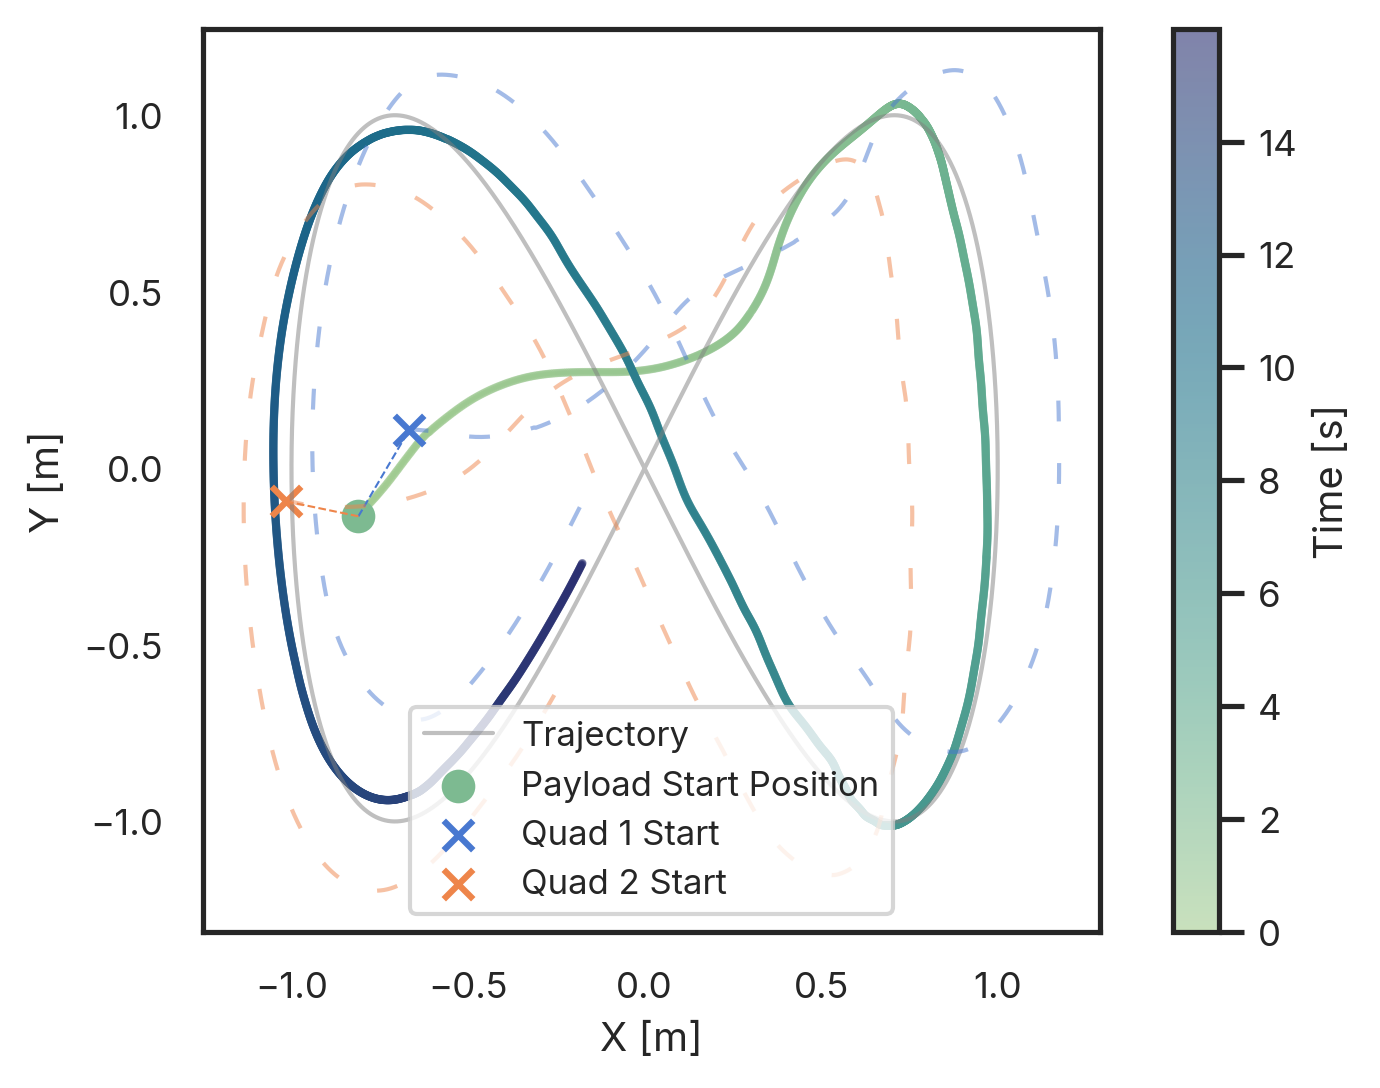
\includegraphics[width=\textwidth]{experiments/payload_position_xy.png}
        \caption{3 agents: figure-eight tracking.}
        \label{fig:payload_position_3quads}
    \end{subfigure}

    \vspace{1em}

    % Five quadrotors
    \begin{subfigure}[b]{0.49\textwidth}
        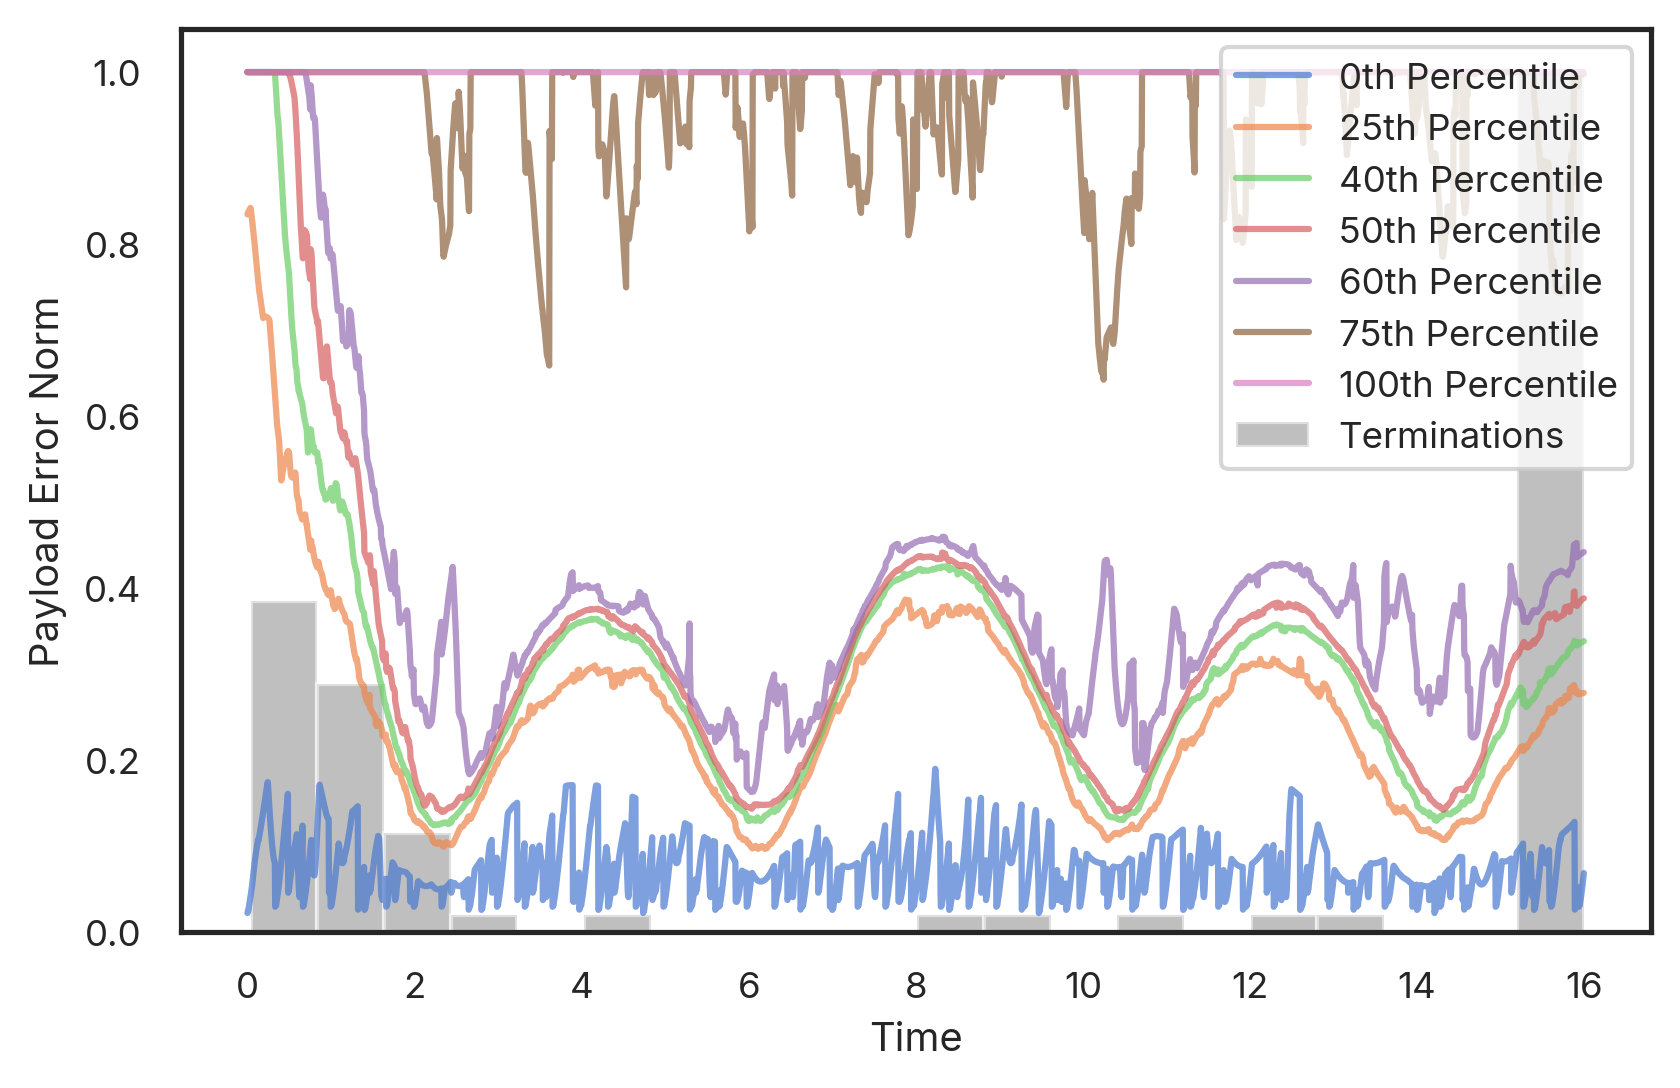
\includegraphics[width=\textwidth]{experiments/payload_error_over_time.png}
        \caption{5 agents: positional error over time (1,000 rollouts).}
        \label{fig:payload_error_5quads}
    \end{subfigure}
    \hfill
    \begin{subfigure}[b]{0.49\textwidth}
        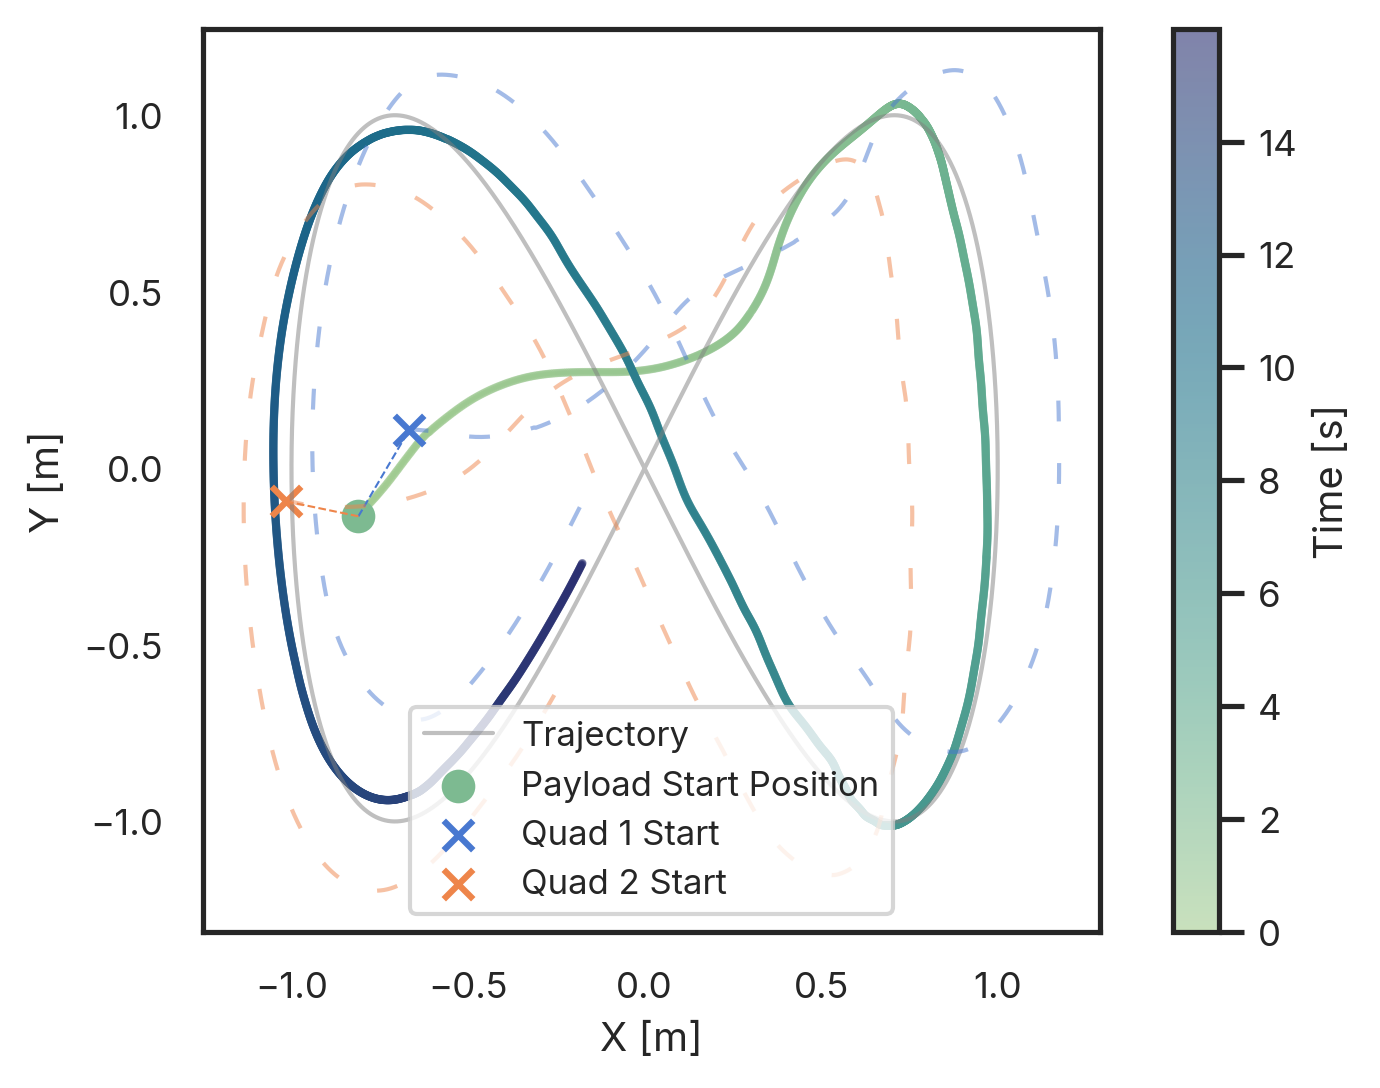
\includegraphics[width=\textwidth]{experiments/payload_position_xy.png}
        \caption{5 agents: figure-eight tracking.}
        \label{fig:payload_position_5quads}
    \end{subfigure}

    \caption{Cooperative payload transport with 2, 3, and 5 quadrotors: error attenuation (left) and trajectory fidelity (right).}
    \label{fig:multi_quad_payload}
\end{figure}

% optional
\section{Comparison with classic control}
Compare with prev paper method \autocite{Wahba2024}
\begin{itemize}
    \item Plots Traj: Trajectory following 3d, error over time for batch
    \item Plots Disturbance: Trajectory following with disturbance, error over time for batch
    \item Plots ground start: Trajectory following with disturbance, error over time for batch
\end{itemize} 
\section{Sim-to-Real Transfer}
\begin{itemize}
    \item one and three quads
    \item Plots Traj: Trajectory following 3d,  error over time 
    \item Plots Disturbance: Position holding with disturbance
\end{itemize}

\section{Generalization}
Does it generalize to different payloads?

\section{Ablation Studies}
\begin{itemize}
    \item Ablation on reward design
    \item Ablation on training parameters
    \item Ablation on domain randomization
    
\end{itemize}